\section{Spacecraft Modes of Operation}
The spacecraft will experience the following modes during its lifetime. A different configuration of system operations and instructions will be executed by \textit{SnapSat} in each case. These are summarised in table~\ref{tab:modesofoperation} below.

\begin{table}[H]
    \centering
    \caption{SnapSat Modes of Operation}
    \vspace{0.15cm}
    \label{tab:modesofoperation}
    {\renewcommand{\arraystretch}{1.4}%
        \begin{tabular}{|>{\arraybackslash}m{4.5cm}|>{\arraybackslash}m{10.5cm}|}
            \hline
            \textbf{Spacecraft Mode} & \textbf{Description} \\ \hline\hline
            Launch Mode &  This turns the satellite off for launch to comply with CubeSat Design Specification 2.3.1. During launch the deployment switch is tripped which will turn the satellite on and transfer it into Establish Contact Mode.
            \\\hline
            Safe mode & (NOTE: this is example text) This mode is intended to keep the satellite alive. Only the essential components are ON all the time - such as the OBC, power board and VHF receiver. Transmitter is turned ON occasionally. 
            Has uncontrolled attitude. 
             \\\hline
            Recovery/De-tumble mode & (NOTE: this is example text) This mode is used to de-tumble the spacecraft after ejection from the deployment dispenser as well as to recover it from any spin-ups. In addition to the essential components that are ON all the time, the ADCS is also operational during this mode. Any other device could be turned ON by ground command.  
            \\\hline
			Establish Contact Mode & In this mode the satellite waits 30 seconds (specifications) before deploying the antenna and attempting to communicate with the ground station
            \\\hline
            Payload Operation Mode & This mode is used only when taking a picture.  The camera module is booted up, the camera takes a picture, stores it is RAM/ROM and then the camera is powered town again to conserve power.  This mode can be triggered by reaching a preset GPS location or manually via communications.  This mode can be entered either by reaching a GPS coordinate or through ground control command.  It exists this mode straight into Relay Picture Mode.
            \\\hline
            Relay Picture Mode & This mode is entered after Payload Operation Mode and causes the CubeSat to start sending pictures to the ground station. 
            \\\hline
            Relay Picture Mode & In this mode the camera is almost constantly transmitting images taken through the camera.  It exists into Telemetry Mode when the picture has been sent. 
            \\\hline
            Telemetry Mode & In this mode the CubeSat is idle, just displaying basic telemetry.  Attitude controlled.
            \\\hline
            etc. (Other Modes) &   \\\hline
        \end{tabular} } 
\end{table}

\begin{figure}[H]
    \centering
    \caption{SnapSat State Diagram}
    \vspace{0.15cm}
    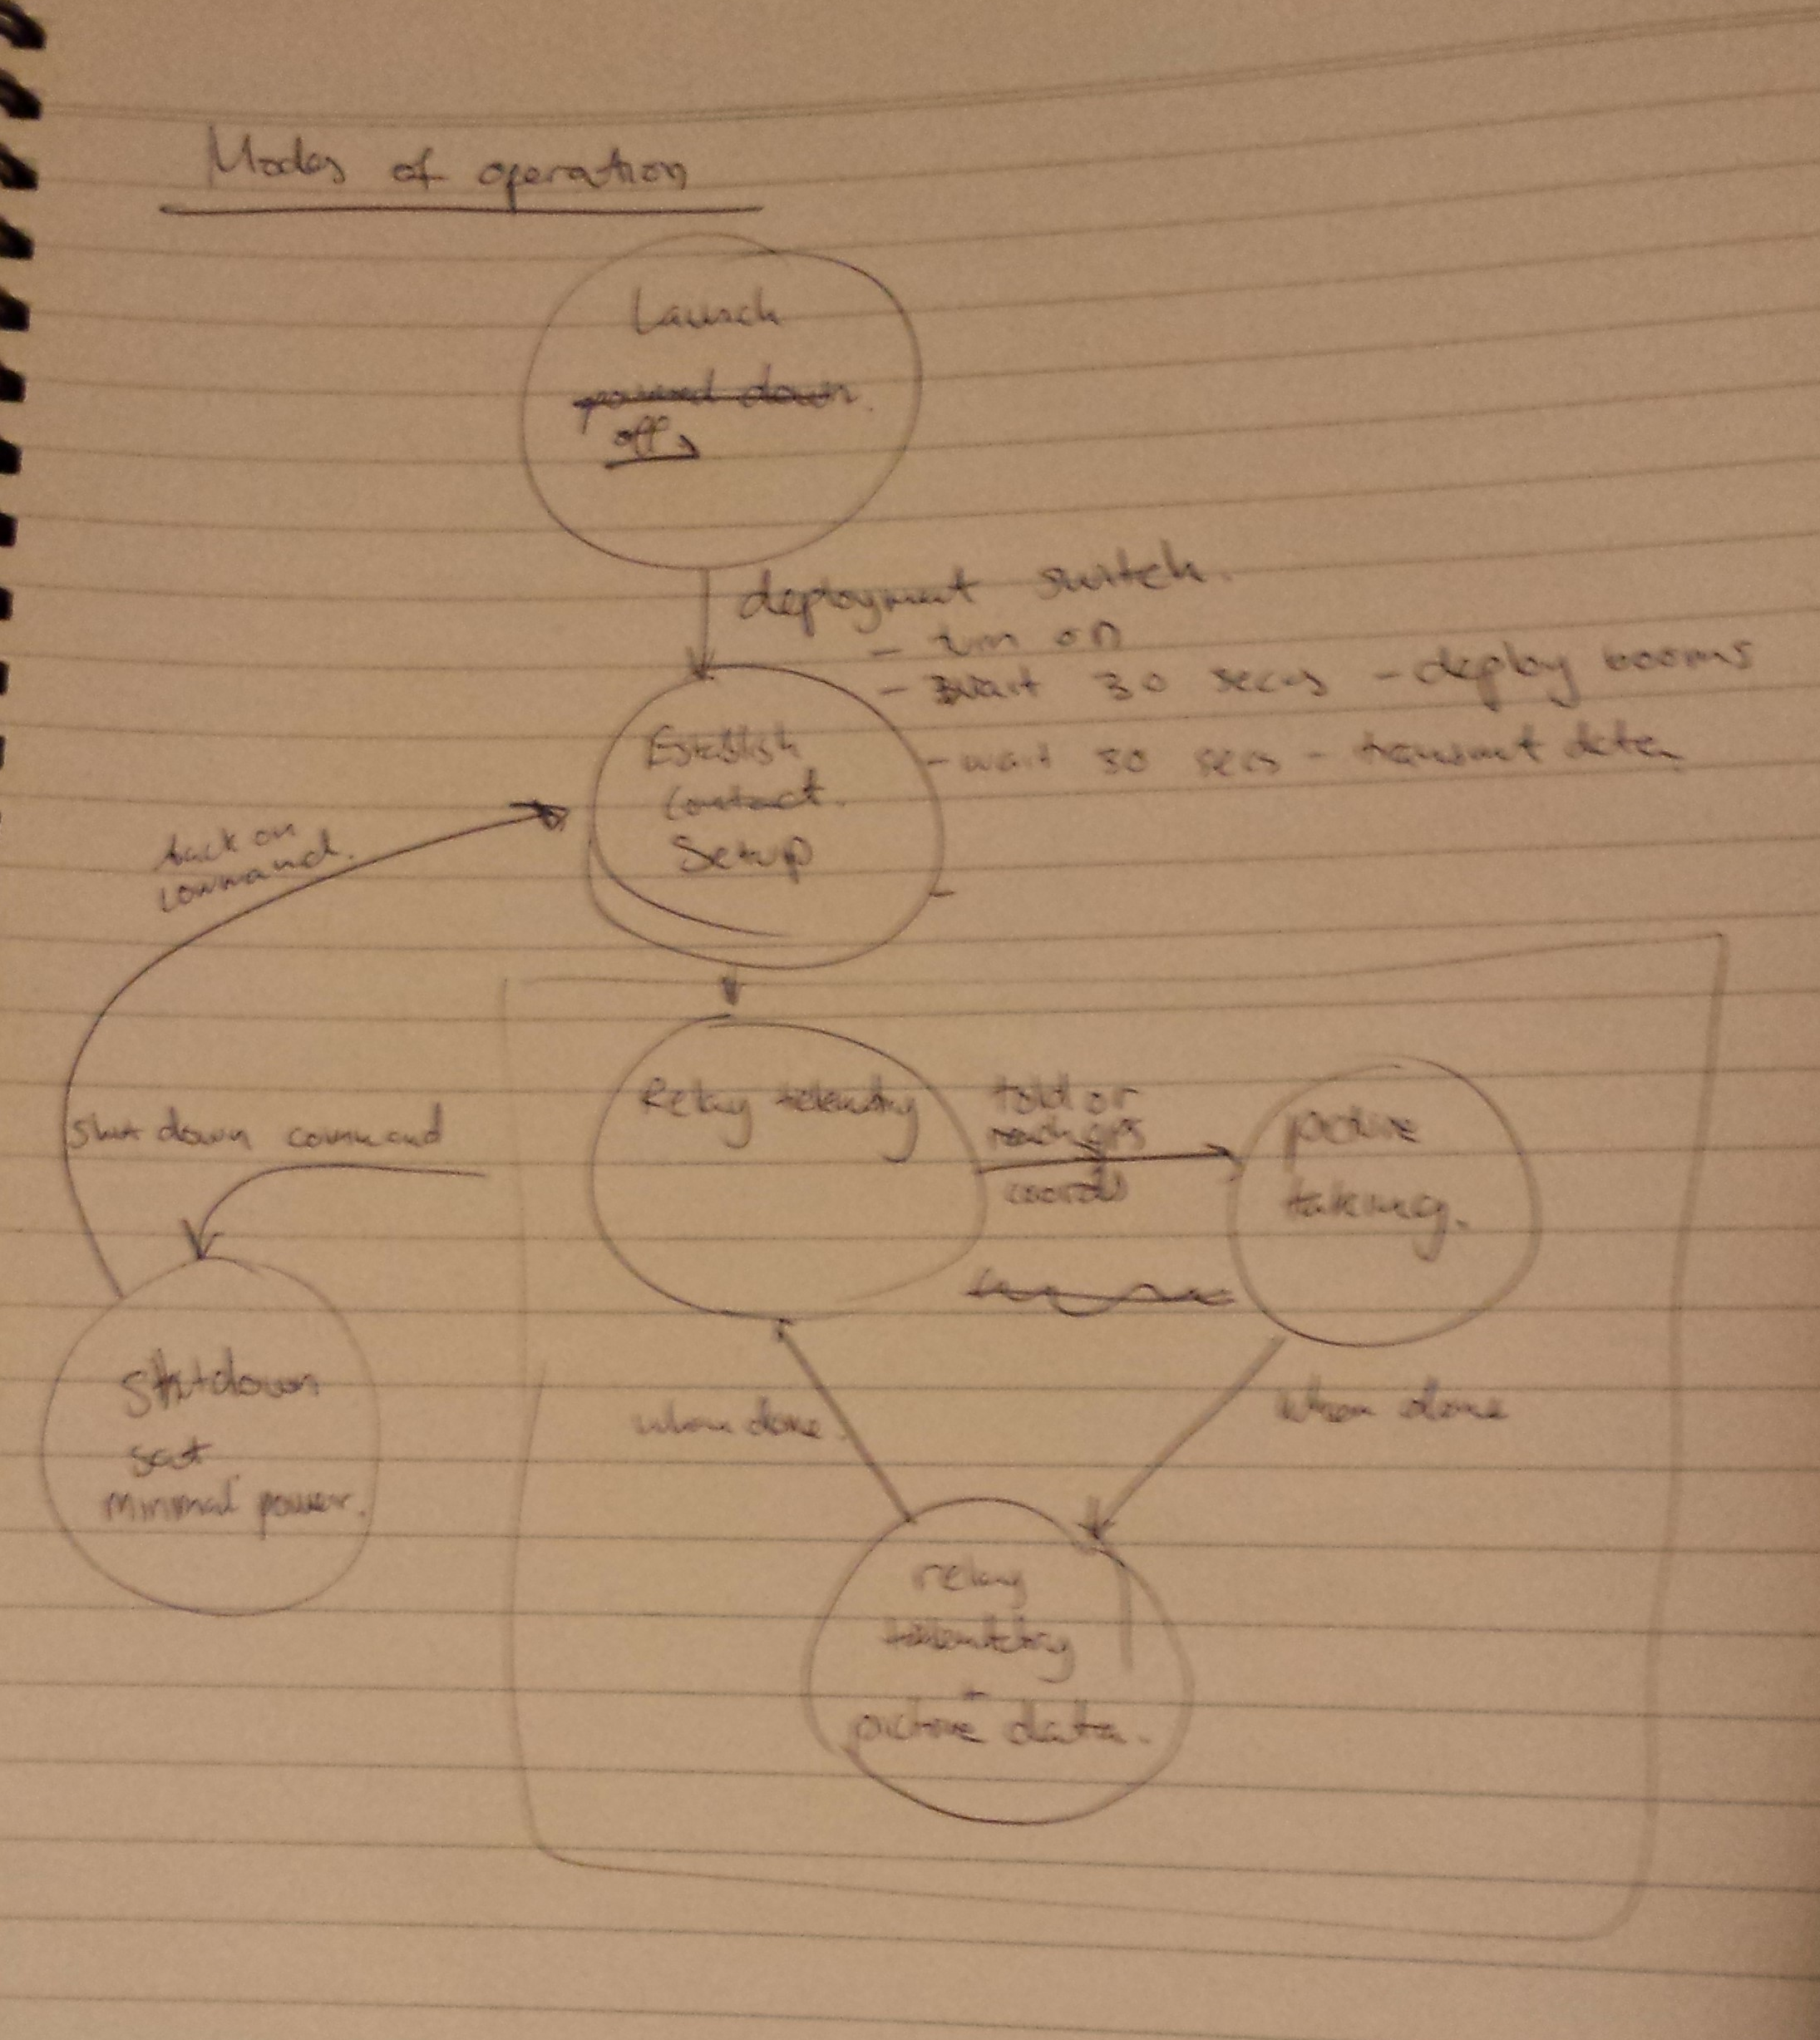
\includegraphics[width=6.5cm]{ModesOfOperation.png}
    \\This diagram illustrates the transitions between states.
\end{figure}